% Options for packages loaded elsewhere
\PassOptionsToPackage{unicode}{hyperref}
\PassOptionsToPackage{hyphens}{url}
\PassOptionsToPackage{dvipsnames,svgnames,x11names}{xcolor}
%
\documentclass[
  letterpaper,
  DIV=11,
  numbers=noendperiod]{scrartcl}

\usepackage{amsmath,amssymb}
\usepackage{iftex}
\ifPDFTeX
  \usepackage[T1]{fontenc}
  \usepackage[utf8]{inputenc}
  \usepackage{textcomp} % provide euro and other symbols
\else % if luatex or xetex
  \usepackage{unicode-math}
  \defaultfontfeatures{Scale=MatchLowercase}
  \defaultfontfeatures[\rmfamily]{Ligatures=TeX,Scale=1}
\fi
\usepackage{lmodern}
\ifPDFTeX\else  
    % xetex/luatex font selection
\fi
% Use upquote if available, for straight quotes in verbatim environments
\IfFileExists{upquote.sty}{\usepackage{upquote}}{}
\IfFileExists{microtype.sty}{% use microtype if available
  \usepackage[]{microtype}
  \UseMicrotypeSet[protrusion]{basicmath} % disable protrusion for tt fonts
}{}
\makeatletter
\@ifundefined{KOMAClassName}{% if non-KOMA class
  \IfFileExists{parskip.sty}{%
    \usepackage{parskip}
  }{% else
    \setlength{\parindent}{0pt}
    \setlength{\parskip}{6pt plus 2pt minus 1pt}}
}{% if KOMA class
  \KOMAoptions{parskip=half}}
\makeatother
\usepackage{xcolor}
\setlength{\emergencystretch}{3em} % prevent overfull lines
\setcounter{secnumdepth}{-\maxdimen} % remove section numbering
% Make \paragraph and \subparagraph free-standing
\ifx\paragraph\undefined\else
  \let\oldparagraph\paragraph
  \renewcommand{\paragraph}[1]{\oldparagraph{#1}\mbox{}}
\fi
\ifx\subparagraph\undefined\else
  \let\oldsubparagraph\subparagraph
  \renewcommand{\subparagraph}[1]{\oldsubparagraph{#1}\mbox{}}
\fi

\usepackage{color}
\usepackage{fancyvrb}
\newcommand{\VerbBar}{|}
\newcommand{\VERB}{\Verb[commandchars=\\\{\}]}
\DefineVerbatimEnvironment{Highlighting}{Verbatim}{commandchars=\\\{\}}
% Add ',fontsize=\small' for more characters per line
\usepackage{framed}
\definecolor{shadecolor}{RGB}{241,243,245}
\newenvironment{Shaded}{\begin{snugshade}}{\end{snugshade}}
\newcommand{\AlertTok}[1]{\textcolor[rgb]{0.68,0.00,0.00}{#1}}
\newcommand{\AnnotationTok}[1]{\textcolor[rgb]{0.37,0.37,0.37}{#1}}
\newcommand{\AttributeTok}[1]{\textcolor[rgb]{0.40,0.45,0.13}{#1}}
\newcommand{\BaseNTok}[1]{\textcolor[rgb]{0.68,0.00,0.00}{#1}}
\newcommand{\BuiltInTok}[1]{\textcolor[rgb]{0.00,0.23,0.31}{#1}}
\newcommand{\CharTok}[1]{\textcolor[rgb]{0.13,0.47,0.30}{#1}}
\newcommand{\CommentTok}[1]{\textcolor[rgb]{0.37,0.37,0.37}{#1}}
\newcommand{\CommentVarTok}[1]{\textcolor[rgb]{0.37,0.37,0.37}{\textit{#1}}}
\newcommand{\ConstantTok}[1]{\textcolor[rgb]{0.56,0.35,0.01}{#1}}
\newcommand{\ControlFlowTok}[1]{\textcolor[rgb]{0.00,0.23,0.31}{#1}}
\newcommand{\DataTypeTok}[1]{\textcolor[rgb]{0.68,0.00,0.00}{#1}}
\newcommand{\DecValTok}[1]{\textcolor[rgb]{0.68,0.00,0.00}{#1}}
\newcommand{\DocumentationTok}[1]{\textcolor[rgb]{0.37,0.37,0.37}{\textit{#1}}}
\newcommand{\ErrorTok}[1]{\textcolor[rgb]{0.68,0.00,0.00}{#1}}
\newcommand{\ExtensionTok}[1]{\textcolor[rgb]{0.00,0.23,0.31}{#1}}
\newcommand{\FloatTok}[1]{\textcolor[rgb]{0.68,0.00,0.00}{#1}}
\newcommand{\FunctionTok}[1]{\textcolor[rgb]{0.28,0.35,0.67}{#1}}
\newcommand{\ImportTok}[1]{\textcolor[rgb]{0.00,0.46,0.62}{#1}}
\newcommand{\InformationTok}[1]{\textcolor[rgb]{0.37,0.37,0.37}{#1}}
\newcommand{\KeywordTok}[1]{\textcolor[rgb]{0.00,0.23,0.31}{#1}}
\newcommand{\NormalTok}[1]{\textcolor[rgb]{0.00,0.23,0.31}{#1}}
\newcommand{\OperatorTok}[1]{\textcolor[rgb]{0.37,0.37,0.37}{#1}}
\newcommand{\OtherTok}[1]{\textcolor[rgb]{0.00,0.23,0.31}{#1}}
\newcommand{\PreprocessorTok}[1]{\textcolor[rgb]{0.68,0.00,0.00}{#1}}
\newcommand{\RegionMarkerTok}[1]{\textcolor[rgb]{0.00,0.23,0.31}{#1}}
\newcommand{\SpecialCharTok}[1]{\textcolor[rgb]{0.37,0.37,0.37}{#1}}
\newcommand{\SpecialStringTok}[1]{\textcolor[rgb]{0.13,0.47,0.30}{#1}}
\newcommand{\StringTok}[1]{\textcolor[rgb]{0.13,0.47,0.30}{#1}}
\newcommand{\VariableTok}[1]{\textcolor[rgb]{0.07,0.07,0.07}{#1}}
\newcommand{\VerbatimStringTok}[1]{\textcolor[rgb]{0.13,0.47,0.30}{#1}}
\newcommand{\WarningTok}[1]{\textcolor[rgb]{0.37,0.37,0.37}{\textit{#1}}}

\providecommand{\tightlist}{%
  \setlength{\itemsep}{0pt}\setlength{\parskip}{0pt}}\usepackage{longtable,booktabs,array}
\usepackage{calc} % for calculating minipage widths
% Correct order of tables after \paragraph or \subparagraph
\usepackage{etoolbox}
\makeatletter
\patchcmd\longtable{\par}{\if@noskipsec\mbox{}\fi\par}{}{}
\makeatother
% Allow footnotes in longtable head/foot
\IfFileExists{footnotehyper.sty}{\usepackage{footnotehyper}}{\usepackage{footnote}}
\makesavenoteenv{longtable}
\usepackage{graphicx}
\makeatletter
\def\maxwidth{\ifdim\Gin@nat@width>\linewidth\linewidth\else\Gin@nat@width\fi}
\def\maxheight{\ifdim\Gin@nat@height>\textheight\textheight\else\Gin@nat@height\fi}
\makeatother
% Scale images if necessary, so that they will not overflow the page
% margins by default, and it is still possible to overwrite the defaults
% using explicit options in \includegraphics[width, height, ...]{}
\setkeys{Gin}{width=\maxwidth,height=\maxheight,keepaspectratio}
% Set default figure placement to htbp
\makeatletter
\def\fps@figure{htbp}
\makeatother

\KOMAoption{captions}{tableheading}
\makeatletter
\@ifpackageloaded{tcolorbox}{}{\usepackage[skins,breakable]{tcolorbox}}
\@ifpackageloaded{fontawesome5}{}{\usepackage{fontawesome5}}
\definecolor{quarto-callout-color}{HTML}{909090}
\definecolor{quarto-callout-note-color}{HTML}{0758E5}
\definecolor{quarto-callout-important-color}{HTML}{CC1914}
\definecolor{quarto-callout-warning-color}{HTML}{EB9113}
\definecolor{quarto-callout-tip-color}{HTML}{00A047}
\definecolor{quarto-callout-caution-color}{HTML}{FC5300}
\definecolor{quarto-callout-color-frame}{HTML}{acacac}
\definecolor{quarto-callout-note-color-frame}{HTML}{4582ec}
\definecolor{quarto-callout-important-color-frame}{HTML}{d9534f}
\definecolor{quarto-callout-warning-color-frame}{HTML}{f0ad4e}
\definecolor{quarto-callout-tip-color-frame}{HTML}{02b875}
\definecolor{quarto-callout-caution-color-frame}{HTML}{fd7e14}
\makeatother
\makeatletter
\makeatother
\makeatletter
\makeatother
\makeatletter
\@ifpackageloaded{caption}{}{\usepackage{caption}}
\AtBeginDocument{%
\ifdefined\contentsname
  \renewcommand*\contentsname{Table of contents}
\else
  \newcommand\contentsname{Table of contents}
\fi
\ifdefined\listfigurename
  \renewcommand*\listfigurename{List of Figures}
\else
  \newcommand\listfigurename{List of Figures}
\fi
\ifdefined\listtablename
  \renewcommand*\listtablename{List of Tables}
\else
  \newcommand\listtablename{List of Tables}
\fi
\ifdefined\figurename
  \renewcommand*\figurename{Figure}
\else
  \newcommand\figurename{Figure}
\fi
\ifdefined\tablename
  \renewcommand*\tablename{Table}
\else
  \newcommand\tablename{Table}
\fi
}
\@ifpackageloaded{float}{}{\usepackage{float}}
\floatstyle{ruled}
\@ifundefined{c@chapter}{\newfloat{codelisting}{h}{lop}}{\newfloat{codelisting}{h}{lop}[chapter]}
\floatname{codelisting}{Listing}
\newcommand*\listoflistings{\listof{codelisting}{List of Listings}}
\makeatother
\makeatletter
\@ifpackageloaded{caption}{}{\usepackage{caption}}
\@ifpackageloaded{subcaption}{}{\usepackage{subcaption}}
\makeatother
\makeatletter
\@ifpackageloaded{tcolorbox}{}{\usepackage[skins,breakable]{tcolorbox}}
\makeatother
\makeatletter
\@ifundefined{shadecolor}{\definecolor{shadecolor}{rgb}{.97, .97, .97}}
\makeatother
\makeatletter
\makeatother
\makeatletter
\makeatother
\ifLuaTeX
  \usepackage{selnolig}  % disable illegal ligatures
\fi
\IfFileExists{bookmark.sty}{\usepackage{bookmark}}{\usepackage{hyperref}}
\IfFileExists{xurl.sty}{\usepackage{xurl}}{} % add URL line breaks if available
\urlstyle{same} % disable monospaced font for URLs
\hypersetup{
  pdftitle={Webscraping Tables},
  pdfauthor={Emily Malcolm-White},
  colorlinks=true,
  linkcolor={blue},
  filecolor={Maroon},
  citecolor={Blue},
  urlcolor={Blue},
  pdfcreator={LaTeX via pandoc}}

\title{Webscraping Tables}
\author{Emily Malcolm-White}
\date{}

\begin{document}
\maketitle
\ifdefined\Shaded\renewenvironment{Shaded}{\begin{tcolorbox}[boxrule=0pt, sharp corners, borderline west={3pt}{0pt}{shadecolor}, breakable, enhanced, interior hidden, frame hidden]}{\end{tcolorbox}}\fi


\includegraphics[width=0.3\textwidth,height=\textheight]{118_N_webscraping_tables_files/mediabag/logo.png}

\begin{Shaded}
\begin{Highlighting}[]
\CommentTok{\#LOAD PACKAGES }
\FunctionTok{library}\NormalTok{(tidyverse)}
\end{Highlighting}
\end{Shaded}

Data doesn't just magically appear on your computer you need to get it
from somewhere.

Sometimes we download data files (\texttt{.csv}, \texttt{.xlsx}, etc.)
and save them locally. Other times, we use datasets that come bundled
with R packages (like the \texttt{gapminder} dataset).

\hypertarget{obtaining-data-from-the-web}{%
\section{Obtaining Data From The
Web}\label{obtaining-data-from-the-web}}

Say you're interested in renting an apartment in Vermont---or studying
the rental market. You might browse Craigslist's Vermont rental
listings.

You could spend hours copying and pasting each listing\ldots{} or you
could write code that extracts the data for you.

When you visit a website, your browser loads the HTML source code, which
includes the structure and content of the page---like headings, tables,
and links. We can use R to read that code and extract specific content.
This is called web scraping.

\hypertarget{should-we-be-scraping-this-data}{%
\section{🛑 Should we be scraping this
data?}\label{should-we-be-scraping-this-data}}

Before scraping, always ask:

\begin{itemize}
\tightlist
\item
  Is it legal?
\item
  Can your specific use case violate the rules?
\item
  Even if legal, is it ethical?
\end{itemize}

In the U.S., scraping public data is typically legal if:

\begin{itemize}
\tightlist
\item
  It's not used for harmful purposes
\item
  It doesn't interfere with a website's business
\item
  It excludes personally identifiable information (PII)
\end{itemize}

\hypertarget{case-law-examples}{%
\section{Case Law Examples}\label{case-law-examples}}

\begin{itemize}
\tightlist
\item
  \href{https://en.wikipedia.org/wiki/EBay_v._Bidder\textquotesingle{}s_Edge\#Order}{eBay
  vs.~Bidder's Edge (2000)}: Bots restricted from overloading systems
\item
  \href{https://en.wikipedia.org/wiki/Facebook,_Inc._v._Power_Ventures,_Inc.\#Ruling}{Facebook
  vs.~Power Venures (2009)}: Logging in on others' behalf violated terms
\item
  \href{https://en.wikipedia.org/wiki/HiQ_Labs_v._LinkedIn}{Linkedin
  vs.~hiQ Labs (2019)}: Scraping public profiles ruled permissible
\end{itemize}

Websites often describe scraping policies in two places:

\begin{enumerate}
\def\labelenumi{\arabic{enumi}.}
\tightlist
\item
  Their robots.txt file (e.g., craigslist.org/robots.txt)
\item
  Their Terms of Service (TOS) document
\end{enumerate}

Craigslist explicitly forbids scraping. Wikipedia does not.

\begin{tcolorbox}[enhanced jigsaw, toprule=.15mm, colbacktitle=quarto-callout-note-color!10!white, breakable, bottomtitle=1mm, leftrule=.75mm, arc=.35mm, coltitle=black, opacitybacktitle=0.6, opacityback=0, bottomrule=.15mm, colframe=quarto-callout-note-color-frame, toptitle=1mm, colback=white, left=2mm, titlerule=0mm, title=\textcolor{quarto-callout-note-color}{\faInfo}\hspace{0.5em}{Note}, rightrule=.15mm]

Why might Craigslist restrict scraping, while Wikipedia allows it?

\end{tcolorbox}

\hypertarget{how-does-html-work}{%
\section{How does HTML work?}\label{how-does-html-work}}

HTML (HyperText Markup Language) is the language used to create web
pages. HTML uses tags (like \texttt{\textless{}table\textgreater{}},
\texttt{\textless{}tr\textgreater{}},
\texttt{\textless{}td\textgreater{}}) to define page elements. If we
understand this structure, we can write code that extracts tables and
other elements from the page.

\begin{tcolorbox}[enhanced jigsaw, toprule=.15mm, colbacktitle=quarto-callout-tip-color!10!white, breakable, bottomtitle=1mm, leftrule=.75mm, arc=.35mm, coltitle=black, opacitybacktitle=0.6, opacityback=0, bottomrule=.15mm, colframe=quarto-callout-tip-color-frame, toptitle=1mm, colback=white, left=2mm, titlerule=0mm, title=\textcolor{quarto-callout-tip-color}{\faLightbulb}\hspace{0.5em}{Tip}, rightrule=.15mm]

Typically, an HTML element is defined by a start tag, some content, and
an end tag

\texttt{\textless{}tagname\textgreater{}\ ...some\ content\ here...\ \textless{}/tagname\textgreater{}}

\end{tcolorbox}

For example:

\begin{verbatim}
<html>
<head>
<title>Page Title</title>
</head>
<body>

<h1>My First Heading</h1>
<p>My first paragraph.</p>

</body>
</html>
\end{verbatim}

There are many, many different possible tag elements. In this class,
it's not important that you know the specifics of what each element is.
It's useful for you to understand the basic structure.

\hypertarget{html-tables}{%
\subsection{HTML Tables}\label{html-tables}}

An HTML table is used to represent data in a structured way

\begin{itemize}
\tightlist
\item
  \texttt{\textless{}table\textgreater{}} Defines a table
\item
  \texttt{\textless{}th\textgreater{}} Defines a header cell in a table
\item
  \texttt{\textless{}tr\textgreater{}} Defines a row in a table
\item
  \texttt{\textless{}td\textgreater{}} Defines a cell in a table
\end{itemize}

Here is the HTML code:

\begin{verbatim}
<table>
  <tr>
    <th>Name</th>
    <th>Birth Year</th>  
    <th>Country</th>
  </tr>
  <tr>
    <td>Harry Styles</td>
    <td>Feb 1, 1994</td>
    <td>Britain</td>
  </tr>
  <tr>
    <td>Taylor Swift</td>
    <td>Dec 13, 1989</td>
    <td>USA</td>
  </tr>
  <tr>
    <td>Justin Bieber</td>
    <td>Mar 1, 1994</td>
    <td>Canada</td>
  </tr>
</table>
\end{verbatim}

Here is how the HTML displays in a web browser:

Name

Birth Year

Country

Harry Styles

Feb 1, 1994

Britain

Taylor Swift

Dec 13, 1989

USA

Justin Bieber

Mar 1, 1994

Canada

Today's class will focus on scraping data from HTML tables!

\hypertarget{html-class}{%
\subsection{HTML class}\label{html-class}}

The \texttt{class} attribute can be added to any HTML element. Often it
is used to help customize the styling of the element (among other
things).

\begin{verbatim}
<h2 class="city">Middlebury</h2>
<p class="city">Middlebury is a town in Vermont</p>
\end{verbatim}

This can be particularly useful in web scraping -- we can ask to scrape
particular elements, particular classes, or both!

\hypertarget{web-scraping-using-rvest}{%
\section{\texorpdfstring{Web Scraping using
\texttt{rvest}}{Web Scraping using rvest}}\label{web-scraping-using-rvest}}

We need the package \href{https://rvest.tidyverse.org/}{\texttt{rvest}}
to help us with this.

\begin{Shaded}
\begin{Highlighting}[]
\FunctionTok{library}\NormalTok{(rvest)}
\end{Highlighting}
\end{Shaded}

\hypertarget{viewing-raw-html-from-a-website}{%
\subsection{Viewing Raw HTML from a
website}\label{viewing-raw-html-from-a-website}}

You can inspect the source code of any webpage by using a web browser
like Firefox or Chrome.

\begin{itemize}
\tightlist
\item
  On Firefox, navigate to the ``Tools'' menu item in the top menu and
  click on ``Web Developer/Page Source''. You can also use the shortcut
  \texttt{Command\ +\ U}
\item
  On Chrome, navigate to the top menu item ``View'' and click on
  ``Developer/View Source.'' You can also use the keyboard shortcut
  \texttt{Option-Command-U}. It also can be useful to use the
  \href{https://chrome.google.com/webstore/detail/selectorgadget/mhjhnkcfbdhnjickkkdbjoemdmbfginb/related}{SelectorGadget
  Extension}.
\end{itemize}

\hypertarget{webscraping-tables-from-wikipedia}{%
\subsection{Webscraping Tables from
Wikipedia}\label{webscraping-tables-from-wikipedia}}

Check out the information on the (List of the Most Viewed YouTube Videos
on
Wikipedia){[}https://en.wikipedia.org/wiki/List\_of\_most-viewed\_YouTube\_videos{]}.
Suppose we want to scrape this data to use in R.

\begin{itemize}
\tightlist
\item
  \texttt{read\_html} scrapes the raw html from the webpage as text
\item
  \texttt{html\_element} (and \texttt{html\_elements}) selects
  particular elements from the HTML code
\item
  \texttt{html\_table} formats a scraped html table as a tibble (R
  table)
\end{itemize}

\begin{Shaded}
\begin{Highlighting}[]
\NormalTok{youtube\_videos }\OtherTok{\textless{}{-}} \FunctionTok{read\_html}\NormalTok{(}\StringTok{"https://en.wikipedia.org/wiki/List\_of\_most{-}viewed\_YouTube\_videos"}\NormalTok{) }\SpecialCharTok{\%\textgreater{}\%}
  \FunctionTok{html\_element}\NormalTok{(}\StringTok{".wikitable"}\NormalTok{) }\SpecialCharTok{\%\textgreater{}\%}
  \FunctionTok{html\_table}\NormalTok{() }

\NormalTok{youtube\_videos}
\end{Highlighting}
\end{Shaded}

\begin{verbatim}
# A tibble: 31 x 6
   `Video name`                    Uploader `Views (billions)` Date  Notes ``   
   <chr>                           <chr>    <chr>              <chr> <chr> <chr>
 1 Baby Shark Dance[7]             Pinkfon~ 15.65              June~ "[A]" <NA> 
 2 Despacito[10]                   Luis Fo~ 8.66               Janu~ "[B]" <NA> 
 3 Wheels on the Bus[18]           Cocomel~ 7.17               May ~ ""    <NA> 
 4 Johny Johny Yes Papa[19]        LooLoo ~ 7.02               Octo~ ""    <NA> 
 5 Bath Song[20]                   Cocomel~ 7.01               May ~ ""    <NA> 
 6 See You Again[21]               Wiz Kha~ 6.58               Apri~ "[C]" <NA> 
 7 Shape of You[26]                Ed Shee~ 6.42               Janu~ "[D]" <NA> 
 8 Phonics Song with Two Words[29] ChuChu ~ 6.31               Marc~ ""    <NA> 
 9 Uptown Funk[30]                 Mark Ro~ 5.49               Nove~ ""    <NA> 
10 Gangnam Style[31]               Psy      5.48               July~ "[E]" <NA> 
# i 21 more rows
\end{verbatim}

\begin{itemize}
\item
  We could have used \texttt{html\_element("table")} If we did this, it
  would have pulled the first \texttt{\textless{}table\textgreater{}}
  from the page.
\item
  We could have used \texttt{html\_elements("table")} If we did this, it
  would have pulled all the \texttt{\textless{}table\textgreater{}}
  elements from the page.
\item
  If you want a specific table that isn't the first table, scrape all
  the tables and apply \texttt{html\_table()}. Then take that new object
  of the tables and add \texttt{{[}{[}n{]}{]}} to get the \(n^{th}\)
  table. For example to call the \(2^{nd}\) table,
\end{itemize}

\begin{verbatim}
tables <- html %>% 
  html_elements("table") %>%
  html_table() 
  
tables[[2]]
\end{verbatim}

\begin{itemize}
\tightlist
\item
  In this case, we used \texttt{html\_elements(".wikitable")} I choose
  to use this because the \texttt{\textless{}table\textgreater{}} was
  also defined with a unique \texttt{class}:
  \texttt{\textless{}table\ class="wikitable\ sortable"\textgreater{}}
\end{itemize}

\begin{tcolorbox}[enhanced jigsaw, toprule=.15mm, colbacktitle=quarto-callout-warning-color!10!white, breakable, bottomtitle=1mm, leftrule=.75mm, arc=.35mm, coltitle=black, opacitybacktitle=0.6, opacityback=0, bottomrule=.15mm, colframe=quarto-callout-warning-color-frame, toptitle=1mm, colback=white, left=2mm, titlerule=0mm, title=\textcolor{quarto-callout-warning-color}{\faExclamationTriangle}\hspace{0.5em}{Warning}, rightrule=.15mm]

Note that if we are using \texttt{html\_element} to call a class, it is
important to add a ``\texttt{.}'' before the class element name. You do
not need to do this is you are calling an HTML element (like ``table'')

\end{tcolorbox}

\hypertarget{cleaning-up-with-janitor}{%
\subsection{\texorpdfstring{Cleaning up with
\texttt{janitor}}{Cleaning up with janitor}}\label{cleaning-up-with-janitor}}

Web scraping doesn't always format perfectly. Let's clean it up!

\begin{Shaded}
\begin{Highlighting}[]
\FunctionTok{library}\NormalTok{(janitor)}
\end{Highlighting}
\end{Shaded}

\begin{figure}

{\centering 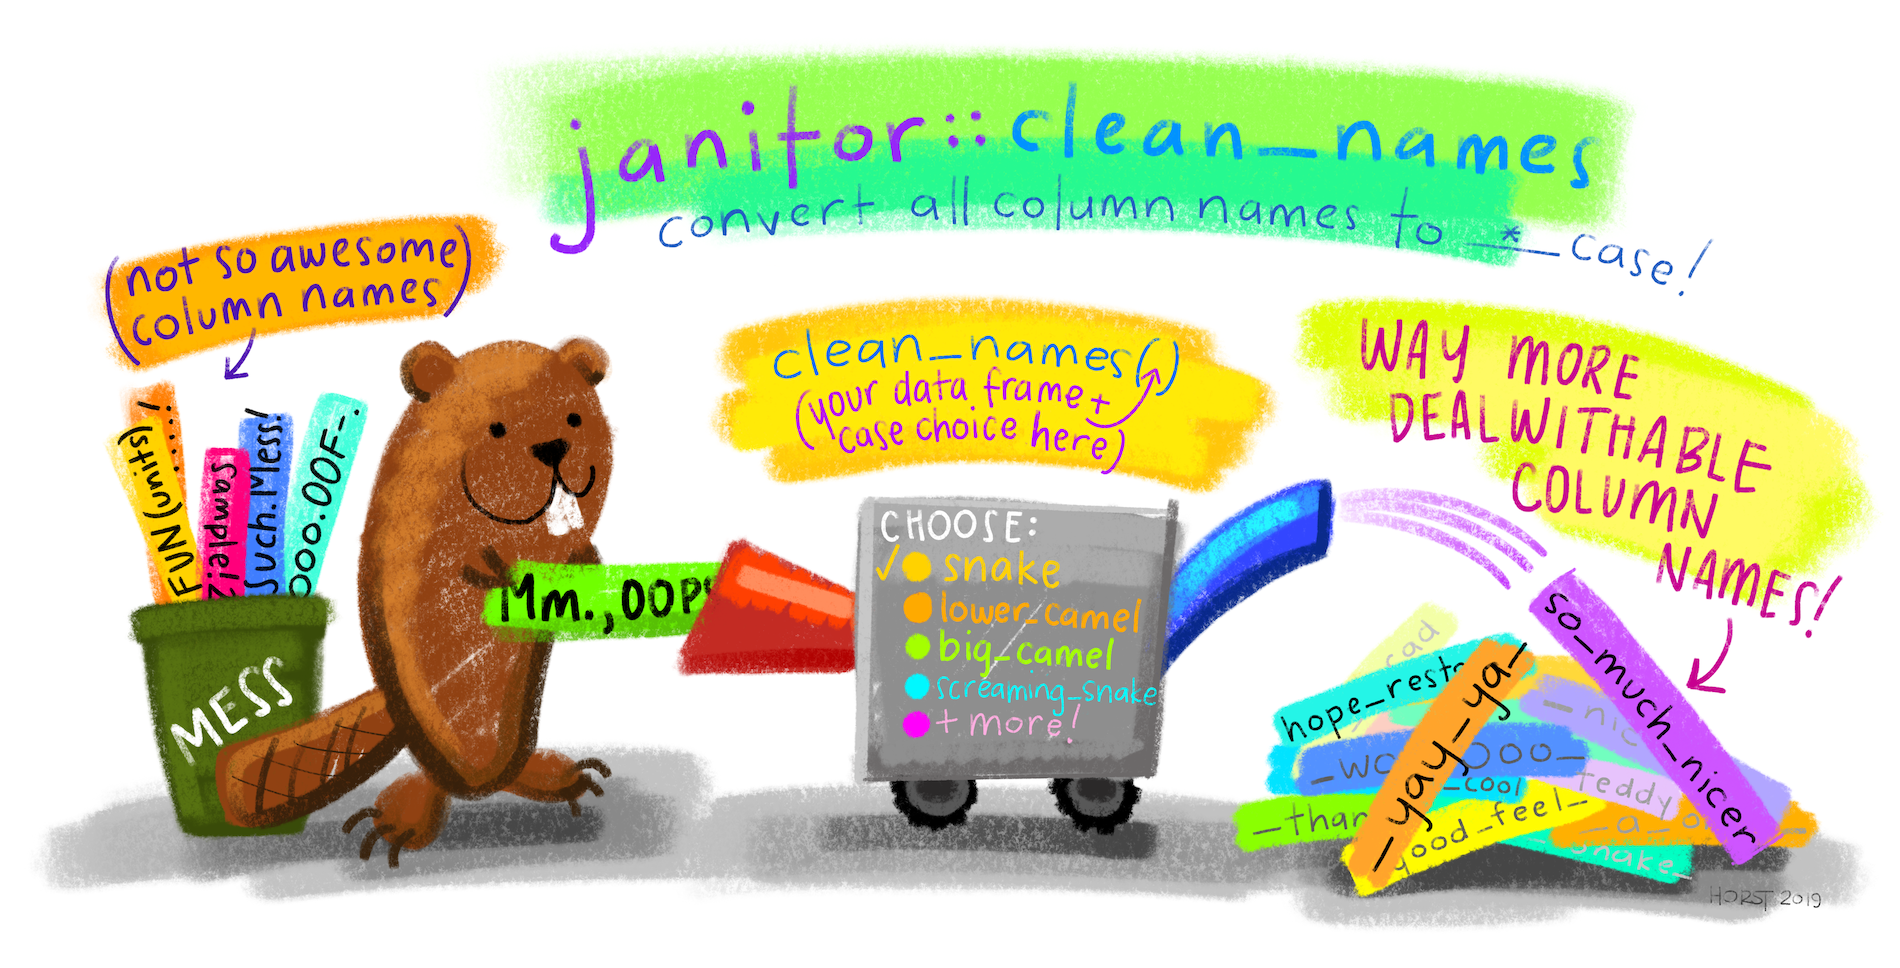
\includegraphics[width=0.5\textwidth,height=\textheight]{118_N_webscraping_tables_files/mediabag/79a12c01-0cc1-4643-b.png}

}

\caption{Artwork by @allisonhorst}

\end{figure}

Clean up the names of the header:

\begin{Shaded}
\begin{Highlighting}[]
\NormalTok{youtube\_videos }\OtherTok{\textless{}{-}} \FunctionTok{clean\_names}\NormalTok{(youtube\_videos)}
\end{Highlighting}
\end{Shaded}

Remove the last row:

\begin{Shaded}
\begin{Highlighting}[]
\CommentTok{\# youtube\_videos \textless{}{-} youtube\_videos \%\textgreater{}\% }
\CommentTok{\#   filter(no != "As of August 8, 2023")}
\end{Highlighting}
\end{Shaded}

Format the views as a number using \texttt{as.numeric}:

\begin{Shaded}
\begin{Highlighting}[]
\NormalTok{youtube\_videos }\OtherTok{\textless{}{-}}\NormalTok{ youtube\_videos }\SpecialCharTok{\%\textgreater{}\%} 
  \FunctionTok{mutate}\NormalTok{(}\AttributeTok{views\_billions =} \FunctionTok{as.numeric}\NormalTok{(views\_billions))}
\end{Highlighting}
\end{Shaded}

What are the top 10 most viewed YouTube Videos?

\begin{Shaded}
\begin{Highlighting}[]
\NormalTok{top10 }\OtherTok{\textless{}{-}}\NormalTok{ youtube\_videos }\SpecialCharTok{\%\textgreater{}\%}
  \FunctionTok{arrange}\NormalTok{(}\FunctionTok{desc}\NormalTok{(views\_billions)) }\SpecialCharTok{\%\textgreater{}\%}
  \FunctionTok{slice}\NormalTok{(}\DecValTok{1}\SpecialCharTok{:}\DecValTok{10}\NormalTok{)}

\NormalTok{top10}
\end{Highlighting}
\end{Shaded}

\begin{verbatim}
# A tibble: 10 x 6
   video_name                      uploader     views_billions date  notes x    
   <chr>                           <chr>                 <dbl> <chr> <chr> <chr>
 1 Baby Shark Dance[7]             Pinkfong Ba~          15.6  June~ "[A]" <NA> 
 2 Despacito[10]                   Luis Fonsi             8.66 Janu~ "[B]" <NA> 
 3 Wheels on the Bus[18]           Cocomelon -~           7.17 May ~ ""    <NA> 
 4 Johny Johny Yes Papa[19]        LooLoo Kids~           7.02 Octo~ ""    <NA> 
 5 Bath Song[20]                   Cocomelon -~           7.01 May ~ ""    <NA> 
 6 See You Again[21]               Wiz Khalifa            6.58 Apri~ "[C]" <NA> 
 7 Shape of You[26]                Ed Sheeran             6.42 Janu~ "[D]" <NA> 
 8 Phonics Song with Two Words[29] ChuChu TV N~           6.31 Marc~ ""    <NA> 
 9 Uptown Funk[30]                 Mark Ronson            5.49 Nove~ ""    <NA> 
10 Gangnam Style[31]               Psy                    5.48 July~ "[E]" <NA> 
\end{verbatim}

Once we have this data, we can make cool plots!

\begin{Shaded}
\begin{Highlighting}[]
\NormalTok{top10 }\SpecialCharTok{\%\textgreater{}\%} 
  \FunctionTok{ggplot}\NormalTok{( }\FunctionTok{aes}\NormalTok{(}\AttributeTok{x=}\NormalTok{views\_billions, }\AttributeTok{y=}\FunctionTok{reorder}\NormalTok{(video\_name, views\_billions))) }\SpecialCharTok{+}
    \FunctionTok{geom\_bar}\NormalTok{(}\AttributeTok{stat=}\StringTok{"identity"}\NormalTok{) }\SpecialCharTok{+}
    \FunctionTok{xlab}\NormalTok{(}\StringTok{"Views (in billions)"}\NormalTok{) }\SpecialCharTok{+}
    \FunctionTok{ylab}\NormalTok{(}\StringTok{"Videos"}\NormalTok{) }\SpecialCharTok{+}
    \FunctionTok{ggtitle}\NormalTok{(}\StringTok{"Top 10 Most Watched YouTube Videos of All Time"}\NormalTok{) }\SpecialCharTok{+}
    \FunctionTok{theme\_minimal}\NormalTok{()}
\end{Highlighting}
\end{Shaded}

\begin{figure}[H]

{\centering 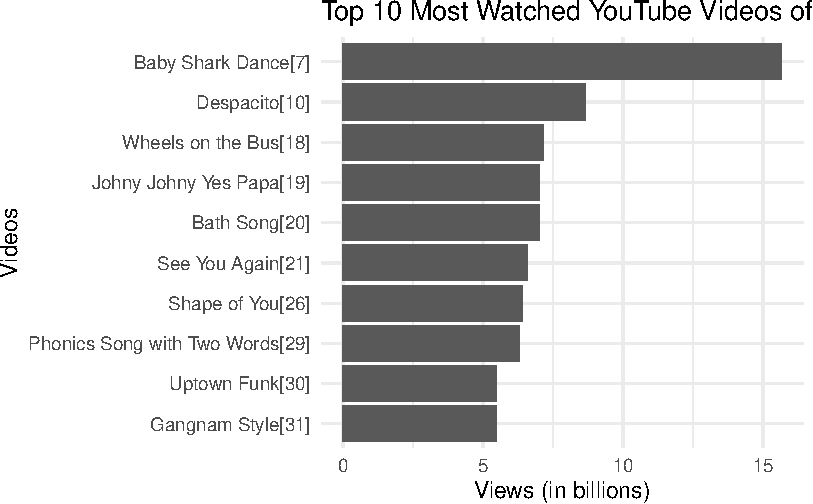
\includegraphics{118_N_webscraping_tables_files/figure-pdf/unnamed-chunk-9-1.pdf}

}

\end{figure}

:::callout-tip In this case, the list of the names is still not
displaying very neatly. For example, rather than
\texttt{"Baby\ Shark\ Dance"{[}6{]}} I might want it to just say
\texttt{Baby\ Shark\ Dance}.

We can use the \texttt{stringr} package to remove symbols and numbers
from the video names. We will be talking more about \texttt{stringr}
later this semester and it's not something I expect you to be able to do
at this point in the semester.

\begin{Shaded}
\begin{Highlighting}[]
\FunctionTok{library}\NormalTok{(stringr)}

\NormalTok{top10 }\SpecialCharTok{\%\textgreater{}\%} 
  \FunctionTok{mutate}\NormalTok{(}\AttributeTok{video\_name=}\FunctionTok{str\_replace\_all}\NormalTok{(video\_name, }\StringTok{"[\^{}[:alpha:]]"}\NormalTok{, }\StringTok{" "}\NormalTok{)) }\SpecialCharTok{\%\textgreater{}\%} 
  \FunctionTok{ggplot}\NormalTok{(}\FunctionTok{aes}\NormalTok{(}\AttributeTok{x=}\NormalTok{views\_billions, }\AttributeTok{y=}\FunctionTok{reorder}\NormalTok{(video\_name, views\_billions))) }\SpecialCharTok{+}
    \FunctionTok{geom\_bar}\NormalTok{(}\AttributeTok{stat=}\StringTok{"identity"}\NormalTok{) }\SpecialCharTok{+}
    \FunctionTok{xlab}\NormalTok{(}\StringTok{"Views (in billions)"}\NormalTok{) }\SpecialCharTok{+}
    \FunctionTok{ylab}\NormalTok{(}\StringTok{"Videos"}\NormalTok{) }\SpecialCharTok{+}
    \FunctionTok{ggtitle}\NormalTok{(}\StringTok{"Top 10 Most Watched YouTube Videos of All Time"}\NormalTok{) }\SpecialCharTok{+}
    \FunctionTok{theme\_minimal}\NormalTok{()}
\end{Highlighting}
\end{Shaded}

\begin{figure}[H]

{\centering 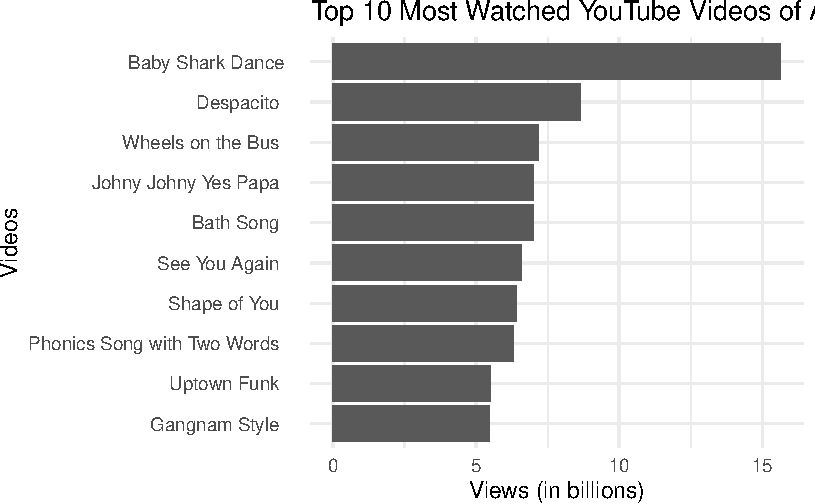
\includegraphics{118_N_webscraping_tables_files/figure-pdf/unnamed-chunk-10-1.pdf}

}

\end{figure}

\begin{tcolorbox}[enhanced jigsaw, toprule=.15mm, opacityback=0, breakable, leftrule=.75mm, colback=white, arc=.35mm, left=2mm, rightrule=.15mm, bottomrule=.15mm]

\textbf{External Resources}\vspace{2mm}

\begin{itemize}
\tightlist
\item
  \href{https://r4ds.hadley.nz/webscraping}{R for Data Science,
  Webscraping}
\end{itemize}

\end{tcolorbox}



\end{document}
